%%%%%%%%%%%%%%%%%%%%%%%%%%%%%%%%%%%%%%%%%
% Presentation Template
% LaTeX Template
% Version 2.0 (2023-06-16)
%
% This template was adapted by:
% Jonathan Decker (jonathan.decker@uni-goettingen.de)
% From a template made by:
% Julian Kunkel (julian.kunkel@gwdg.de)
%
%%%%%%%%%%%%%%%%%%%%%%%%%%%%%%%%%%%%%%%%%
\documentclass[compress,aspectratio=169]{beamer}

% make sure the theme and config files are on this path
% uncomment the required theme setting
\usepackage[GI]{assets/beamerConfig}
%\usepackage[GWDG]{assets/beamerConfig}
%\usepackage[DECICE]{assets/beamerConfig}

\addbibresource{ref.bib}
\graphicspath{{.}{assets/}}

% --- document configuration ---
\newcommand{\mytitle}{What every programmer should know about licenses}
% Leave empty for no subtitle
\newcommand{\mysubtitle}{Create usable code while abiding by the law}
\newcommand{\myauthor}{Lars Quentin}
\newcommand{\myauthorurl}{}
\newcommand{\myvenue}{INFORMATIK 2023}
% For example, use \today
\newcommand{\mydate}{27.09.2023}
% For example, Institute for Computer Science / GWDG
\newcommand{\myinstitute}{GWDG / Campus-Institut Data Science}

\configuretitlepage

\begin{document}

	\begin{frame}[plain]
		\titlepage
	\end{frame}

	\begin{frame}[t]{Table of contents}
		\tableofcontents[subsectionstyle=hide/hide]
	\end{frame}

	% --- slides begin ---

	\section{Introduction}

	\begin{frame}{Learning Goals}
		\begin{itemize}
			\item Why a license is important
      \item How to differentiate between
        \begin{itemize}
          \item Public Domain Licenses
          \item Permissive Licenses
          \item Copyleft Licenses
        \end{itemize}
      \item How to approach non-code licensing
		\end{itemize}
	\end{frame}

	\begin{frame}{Why you should care}
    \begin{block}{What happens if you don't use a license? \cite{nolicense}}
      \begin{itemize}
        \item If a repository has no license, then \textbf{all rights are reserved}!
        \item This means that normal copyright laws apply.
        \item Therefore, nobody is allowed to:
          \begin{itemize}
            \item Copy
            \item Modify
            \item Distribute
          \end{itemize}
        \item If someone else contributes, this includes you!
      \end{itemize}
    \end{block}
    \begin{center}
      \Large If you want to share your code, you need a license!
    \end{center}
	\end{frame}

  \section{Code Licenses}

	\begin{frame}{Overview of Code Licenses}
    Licenses can be divided into three categories:
		\begin{itemize}
      \item Public Domain-like
        \begin{itemize}
          \item The Unlicense
        \end{itemize}
			\item Permissive
        \begin{itemize}
          \item MIT
          \item Apache 2.0
          \item BSD-3-Clause
        \end{itemize}
      \item Copyleft
        \begin{itemize}
          \item GPL
        \end{itemize}
		\end{itemize}
	\end{frame}

  \begin{frame}{Public Domain (Gemeinfreiheit)}
    \begin{columns}
      \begin{column}{0.5\textwidth}
    \begin{itemize}
      \item Releases code into the public domain
      \item Thus, everybody can
        \begin{itemize}
          \item Use (commercially)
          \item Modify
          \item Distribute / Copy / Publish
          \item Sell
        \end{itemize}
      \item No attribution required
      \item Changes can be kept closed-source
      \item Example: The Unlicense \cite{unlicense}
    \end{itemize}
      \end{column}
      \begin{column}{0.5\textwidth}
        \begin{figure}
          
\includegraphics[width=.5\textwidth]{./assets/unlicense.png}
          \caption{Unlicense logo \cite{unlicense}}
        \end{figure}
      \end{column}
    \end{columns}
  \end{frame}

  \begin{frame}{Permissive Licenses}
    \begin{itemize}
      \item Sometimes also called BSD-like \cite{guide}
      \item Also allow everybody to
        \begin{itemize}
          \item Use (commercially)
          \item Modify
          \item Distribute / Copy / Publish
          \item Sell
        \end{itemize}
      \item Requires attribution, at least in the source code
      \item Example licenses:
        \begin{itemize}
          \item MIT: Most commonly used
          \item Apache 2.0 \cite{apache2}: Like MIT, but with a patent clause \cite{apachefaq}
            \begin{itemize}
              \item If you are a contributor with a relevant patent, you grant a license to the patent
            \end{itemize}
          \item BSD-3: Similar to MIT but adds a no-endorsement clause
            \begin{itemize}
              \item If you use our tool, don't use us to endorse or promote your product
            \end{itemize}
        \end{itemize}
    \end{itemize}
  \end{frame}

  \begin{frame}{Copyleft Licenses}
    \begin{columns}
      \begin{column}{0.5\textwidth}
        \begin{itemize}
          \item Allow for any usage and modification
          \item Source has to be made available
          \item Modifications need to have same license
          \item Example: GPLv3
        \end{itemize}
      \end{column}
      \begin{column}{0.5\textwidth}
        \begin{block}{Four Freedoms \cite{freedoms}}
          \begin{enumerate}
            \item Run the program for any purpose
            \item Be able to read the source code
            \item Distribute the program as you wish
            \item Distribute your modified versions
          \end{enumerate}
        \end{block}
      \end{column}
    \end{columns}
  \end{frame}

  \begin{frame}{Copyleft Implications}
    \begin{itemize}
      \item Without copyleft, open source projects can be forked to closed source
        \begin{itemize}
          \item Chromium to Google Chrome (BSD-3)
        \end{itemize}
      \item Without copyleft, people could sell your software
      \item With copyleft, less people can use your software
      \item If React (most popular Web Framework) were GPLv3, those would be open source:
        \begin{itemize}
          \item Facebook
          \item Netflix
          \item Uber
          \item Airbnb
          \item Dropbox
        \end{itemize}
      \item Big projects often need funding, getting funding for open source is hard
        \begin{itemize}
          \item Many succeed, especially in IT infrastructure
        \end{itemize}
    \end{itemize}
  \end{frame}

\section{How to Add a License}

  \begin{frame}
    \begin{columns}
      \begin{column}{0.5\textwidth}
        \begin{block}{How to Add a License}
          \begin{enumerate}
            \item Find License Fulltext
            \item Add name and year if required
            \item Save as \texttt{LICENSE} file in repository
            \item Commit and push to remote
          \end{enumerate}
        \end{block}
      \end{column}
      \begin{column}{0.5\textwidth}
        \begin{figure}
          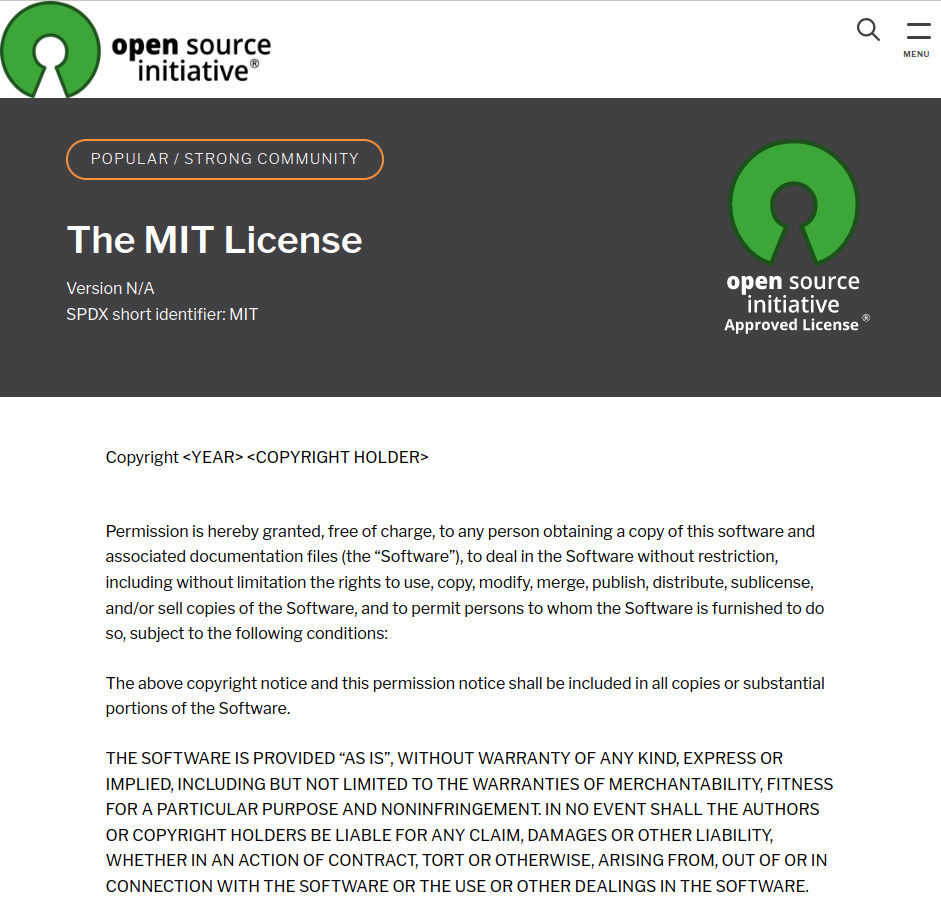
\includegraphics[width=\textwidth]{./assets/mit.png}
          \caption{MIT license from OSI \cite{MITOCI}}
        \end{figure}
      \end{column}
    \end{columns}
  \end{frame}

\section{Non-Code Licenses}

	\begin{frame}{Font Licenses}
    \begin{columns}
      \begin{column}{0.7\textwidth}
		    \begin{itemize}
          \item Most open fonts can be found at Google Fonts \cite{gfonts}
            \begin{itemize}
              \item All of those fonts are licensed permissively
            \end{itemize}
          \item Most used License \cite{gfontsfaq}: SIL Open Font License \cite{ofl}
          \item Other common licenses:
            \begin{itemize}
              \item Apache license \cite{apache2}
              \item Ubuntu Font License \cite{ufl}
            \end{itemize}
		    \end{itemize}
      \end{column}
      \begin{column}{0.3\textwidth}
        \begin{figure}
          
\includegraphics[width=\textwidth]{./assets/gfonts.png}
          \caption{Google Fonts logo \cite{gfonts}}
        \end{figure}
      \end{column}
    \end{columns}
	\end{frame}

  \begin{frame}{Creative Commons Licenses}
    \begin{columns}
      \begin{column}{0.6\textwidth}
		    \begin{itemize}
		    	\item Standardized licenses for creative works
          \item Used for non-code
          \item Can be mapped to code licenses
            \begin{itemize}
              \item Unlicense (Public Domain) $\Rightarrow$ CC0
              \item MIT (Permissive) $\Rightarrow$ CC-BY
              \item GPL (Copyleft) $\Rightarrow$ CC-BY-SA
            \end{itemize}
		    \end{itemize}
      \end{column}
      \begin{column}{0.4\textwidth}
        \begin{figure}
          
\includegraphics[width=\textwidth]{./assets/cc.png}
          \caption{Creative Commons logo \cite{gfonts}}
        \end{figure}
      \end{column}
    \end{columns}
	\end{frame}

  \section{Conclusion}

  \begin{frame}{Conclusion}
		\label{pg:lastpage} % Label on last frame to get the page number for footer
    \begin{block}{Summary}
      \begin{itemize}
        \item Licenses are required so that people can use your work
        \item You can use the following code licenses:
          \begin{itemize}
            \item Public Domain $\Rightarrow$ Unlicense
            \item Permissive $\Rightarrow$ MIT
            \item Copyleft $\Rightarrow$ GPLv3
          \end{itemize}
        \item Use Google Fonts for free fonts
        \item Creative Commons is used for non-code
      \end{itemize}
    \end{block}
  \end{frame}
  \begin{frame}{If you need further help}
      \begin{itemize}
          % \href for functionality, \url for formatting
        \item \href{https://choosealicense.com/}{\url{https://choosealicense.com}}
        \item \href{https://tldrlegal.com/}{\url{https://tldrlegal.com}}
        \item \href{https://www.gnu.org/licenses/license-list.en.html}{\url{https://www.gnu.org/licenses/license-list.en.html}}
        \item \href{https://opensource.org/licenses}{\url{https://opensource.org/licenses}}
        \item \href{https://creativecommons.org/}{\url{https://creativecommons.org/}}
      \end{itemize}
  \end{frame}

	\begin{frame}{References}
		% References slide in appendix
		\renewcommand*{\bibfont}{\normalfont\scriptsize}
		\printbibliography[heading=none]
	\end{frame}

\end{document}
